\section{Computing $\BLap(\Phi)$}
In this section, we propose an Whitening-based Algorithm to compute an approximation $\BLap(\Phi)$ of backbone.

\cite{Par03} proposed an Whitening algorithm which was supposed to determine nodes that always have the same color in all legal colorings of the coloring problem.
This algorithm was also used to compute (non-)frozen literals of model clusters in SAT problem \cite{LMZ09}, from which we can compute (non-)backbone literals.


\begin{algorithm}
\SetKwInOut{Input}{Input}
\SetKwInOut{Output}{Output}
\SetAlgoShortEnd
\SetFillComment
\Input{a formula $\Phi$ and a model $\lambda$ of $\Phi$}
\Output{white clauses $W_c$ and white variables $W_v$}
$W_c:= \{\phi\in\Phi \mid \exists l_1,l_2\in\phi: \  \lambda\models l_1\wedge l_2\}$\;
$W_v:=\{x\in \var(\Phi)\mid \lambda\models x\Rightarrow x\not\in \Lit(\Psi\setminus W_c),
        \ \lambda\models \neg x\Rightarrow \neg x\not\in \Lit(\Psi\setminus W_c)\}$\;
\Repeat{No Update of $W_c$ and $W_v$}{
   $W_c := W_c \cup \{\phi\in\Phi \mid \var(\phi)\cap W_v\neq \emptyset \}$\;
   $W_v := W_v \cup \{x\in \var(\Phi)\mid \lambda\models x\Rightarrow x\not\in \Lit(\Psi\setminus W_c),
        \ \lambda\models \neg x\Rightarrow \neg x\not\in \Lit(\Psi\setminus W_c)\}$
}
\Return $(W_c, W_v)$\;
\caption{Whitening algorithm}
\label{alg:whitening}
\end{algorithm}

Given a satisfiable formula $\Phi$ and a model $\lambda$ of $\Phi$,
Algorithm \ref{alg:whitening} computes a set of white clauses $W_c$ and white variables $W_v$ by iteratively making variables and clauses as white.
Initially, all the clauses which contain at least two satisfied literals by $\lambda$ are marked as white.
Then, all the variables whose values in $\lambda$ do not satisfy any non-white clause are marked as white.
Next, Algorithm \ref{alg:whitening} iteratively and alternatively marks clauses that contain at least one white variable and variables whose values in $\lambda$ do not satisfy any non-white clause are marked as white, until no more clause or variable can be marked as white.
After Algorithm \ref{alg:whitening} has terminated, if a variable $x$ is non-white, i.e., $x\not\in W_v$, then there does not exist
a model $\lambda'\in \cl_\Phi(\lambda)$ such that $\lambda(x)\neq \lambda(x')$. This implies that the literal $x$ (resp. $\neg x$) is a frozen literal
in the model $\lambda$ if $x\in \Lit(\Phi)$ (resp. $\neg x\in \Lit(\Phi)$). We refer to \cite{LMZ09} for details.


Given a satisfiable formula $\Phi$ and a model $\lambda$ of $\Phi$, we use $W_v(\Phi,\lambda)$ (resp. $W_c(\Phi,\lambda)$) to denote the set
$W_v$ (resp. $W_c$) obtained by Algorithm \ref{alg:whitening} taking $\Phi$ and $\lambda$ as inputs, and
$F(\Phi,\lambda)$ to denote the set of literals $\Lit(\Phi)\cap \{x,\neg x\mid x\in \var(\Phi)\setminus W_v(\Phi,\lambda)\}$.



\begin{theorem}\cite{LMZ09}
\label{thm:whiten}
$F(\Phi,\lambda)\subseteq\FL(\Phi,\lambda)$.
\end{theorem}

From Proposition \ref{prop:Frozen-backbone} (i.e., $\BL(\Phi)\subseteq\FL(\Phi,\lambda)$) and Theorem \ref{thm:whiten},
we can get that literals in $F(\Phi,\lambda)$ have high probabilities to be backbone literals. However, the set $F(\Phi,\lambda)$ also contains non-backbone literals. We propose a heuristic strategy that intends to remove non-backbone literals from $F(\Phi,\lambda)$.

\textcolor{red}{Stopped here}
 
 Our strategy is based on the following observation about the relationship between result of Whitening Algorithm and backbone literals:
 Consider the formula $(a\vee\neg b)\wedge(b\vee\neg c)\wedge(c\vee\neg a)$. The backbone of the formula is $\emptyset$. The result of Algorithm \ref{alg:whitening} is $(\emptyset, \emptyset)$. $F(\Phi,\lambda)$ is $\Lit(\Phi)$. However, it's obvious that we can obtain a new model $\lambda(\neg a, \neg b, \neg c)$ from $\lambda$. We construct a dependency graph to recognize such literals like $a,b,c$ from $F(\Phi, \lambda)$ in the given formula automatically.
 
 A dependency graph is a directed graph that describes the adjacent relationship between literals. The literals are the vertexes in the graph. For two literals that in the same clause, there is an edge between them labeled with the clause, for a pair of complementing literals $l$ and $\neg l$, there is an edge between them. For unit clauses, there is a circle edge that pointed back to the literal itself.Intuitively, the literals in unit clauses are backbone literals. Therefore, literals with a circle edge is a backbone literal. Fig \ref{fig:depend} presents an example of dependency graph.
 \begin{figure}
    \centering
    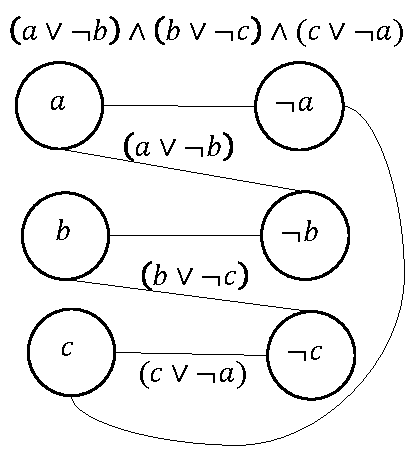
\includegraphics[scale=0.7]{dpendency.pdf}
   \caption{Dependency Graph of $(a\vee\neg b)\wedge(b\vee\neg c)\wedge(c\vee\neg a)$}
   \label{fig:depend}
\end{figure}

 For a path in a dependency graph with a length longer than two, and containing at least two different variables, we call it a \emph{valid path}. Paths that only containing one variable is a trivial path that between a pari of complementing literals. Paths with a length of two is a inside-clause that between two literals in the same clause. Neither of them is useful in recognizing the non-backbone literals automatically.
 
 For valid paths, we want to check the possibility that complementing the literals on paths simultaneously. Given a path $\pi$, we use $\pi[i]$ to denote the $i_{th}$ literal on the path. Suppose a path with a length of four literals, $x, \neg y, y, \neg x$ respectively. It implies that $x$ and $\neg y$ are in the same clause, such as $\phi_1$ and $y, \neg x$ are in the same clause such as $\phi_2$. It's obvious that both $\phi_1$ and $\phi_2$ are still satisfy by the new assignment $\lambda[\neg x, \neg y]$ from the path. The assignment $\lambda[\neg x, \neg y]$ will be a new model if $\Phi_x$ and $\Phi_y$ are either white clauses or clauses labeled in a such path. More generally, if a path with length k, contains several complementing pair of literals started from $\pi[2]$ to $\pi[k-1]$, refereed as \emph{mutate path} then a new assignment $\lambda[\neg l, l\in\{\pi[i] | l\in[2, k-1]\}]$ will satisfy the labeled clauses in this path. If $\Phi_l$, $l\in\{\pi[i] | l\in[2, k-1]\}$ are all white clauses clauses labeled in a mutate path, a new model is obtained from the path. 
 
 Our approach applying the counterexample idea to the facts presented above, consider a literal $l\in F(\Phi, \lambda)$ if there is a non-mutate path starting from $l$, we consider that there is no immediate model generated the literal $l$.
 
 However, it's possible to obtain a new model by complementing the literal that have a non-mutate path. But it's usually time-cost. In order to avoid calling SAT solvers, our approach just remove the literals that have an non-mutate path. We will apply an iteratively SAT testing Algorithm to deal with this literals.


\begin{algorithm}
\SetKwInOut{Input}{Input}
\SetKwInOut{Output}{Output}
\SetAlgoShortEnd
\SetFillComment
\Input{$\Phi$: a formula, $\NBLap$: under-approximation of non-backbone}
\Output{$\BLap(\Phi)$: backbone approximation of $\Phi$}

$\BLap:=F(\Phi, \lambda)\setminus\{l | \forall \pi, \pi[1]==l\Longrightarrow\pi[2k]==\neg\pi[2k+1], k\in[2,n-1]\}$\;
%\For{$l\in\BLap(\Phi)$}{
%    \For{$\phi\in\Phi_l$}{
%        $found:=TRUE$\;
%        $k:=1$\;
%        $\Phi_{l}^0:=\{l\}$\;
%        \Repeat {$\Phi_{l_l}^k==\Phi$}{
%            $\Phi_{l}^k:=\{\phi\in\Phi \mid \neg\Lit(\Phi_{l}^{k-1})\in\phi\}$\;
%            \If{$\neg l\in\Lit(\Phi_{l}^k)$}{
%                    break\;
%            }
%            $k++$\;
%        }
%        \If{$\Phi_{l_l}^k==\Phi$}{
%            $found:=FALSE$\;
%            break\;
%        }
%    }
%    \If{found}{
%        $\BLap(\Phi):=\BLap(\Phi)\setminus\{l\}$\;
%    }
%}
\Return $\BLap(\Phi)$\;
\caption{Backbones approximation of $\Phi$}
\label{alg:nBLo}
\end{algorithm}

